\documentclass{article}
\usepackage[utf8]{inputenc}
\usepackage{authblk}
\usepackage{amsmath}
\usepackage{graphicx}
 \usepackage{setspace}
\doublespacing
\usepackage[style=numeric]{biblatex}
  

\addbibresource{references.bib}




  
      

       \title{Modelling Exciton Diffusion - Final Report}

       
            
       \vspace{1.5cm}
       
       \author{Alfy Benny, Kipp Bradford, Savannah Carnahan,\\ Xiaoqi Chen, and Azmaine Iqtidar}
        \begin{document}
       \maketitle
      
       \vfill
            
       
            
      \vfill
     
       \begin{center}
            
       Software Engineering in Scientific Computing\\
       Princeton University\\
       
    \end{center}    
  
\newpage

\section{Background}

\subsection{Motivation}

Designing, predicting and understanding energy transport in opto-electronic devices and biological systems is a major challenge facing materials science and biology. Exciton transport is a fundamental mode of energy transfer in such systems. Excitons are formed when an electron is excited from its ground state into the conduction band of the material. The exciton is then defined as the quasi-particle formed by the excited electron and the positive hole it left behind. Once an exciton is formed on one molecule, it can then then diffuse to other particles in the system. 

There are two well-established methods for modelling exciton transport.\cite{Oberhofer2017ChargeMethods} In the hopping regime, the particle is viewed as discretely localized on a site in the material. The exciton can then jump from one site to another with a probability depending on the system in question. This approach is best suited to highly disordered materials due to Andersen delocalisation and polaron formation.\cite{DanielBalzer2021DelocalisedMaterials}

In highly ordered materials, the exciton is best modelled as a wave because in these materials the exciton can exist delocalized over several sites.\cite{Oberhofer2017ChargeMethods} It is therefore inaccurate to model the exciton dispersion as existing on discrete sites, and thus, the mobility of the exciton in the material is instead modelled using the velocity of the wavepacket. These two models are quite successful at modelling transports at the extremes; however, many modern materials are in an intermediate zone that is not well described by either model. There are several models that aim to bridge the gap between the models, called the intermediate regime. Our software will primarily focus on modelling the hopping regime, with the goal of having the flexibility to accommodate further advances in models in the field.

\subsection{Theory}

The mechanism of charge transport, regardless of classification is governed by the conductivity of the material $\sigma$:
\begin{align}
    \mathbf{\sigma}=&q\rho_c\mathbf{\mu}
\end{align}

where $q$ is the charge, $\rho_c$ is the density of carriers, and $\mathbf{\mu}$ corresponds to the likelihood that that charge will move in the material (i.e its mobility).\cite{Oberhofer2017ChargeMethods} Both $\mathbf{\mu}$ and $\rho_c$ are dependent on the system being examined. This project is primarily concerned with determining $\mathbf{\mu}$ for a given material with density $\rho_c$. 

In the hopping regime, the probability that an exciton will transfer from site 1 to site 2 is governed in the nonadiabatic limit by the Marcus rate equation:\cite{Marcus1956OnIN}
\begin{align}
    k_{12,nadiab}=&\frac{2\pi}{\hbar}|J_{Coul}|^2\sqrt{\frac{1}{4\pi k_b T \lambda}}e^{-\frac{(\lambda +\Delta G^0)^2}{4\lambda k_b T}}
\end{align}

where $\hbar$ and $k_b$ are constants, $\lambda$ is the reorganization free energy, $J_{Coul}$ is the coupling between the initial site and final site, $\Delta G^0$ is the driving force, and $T$ is the temperature. In the adiabatic limit, this is defined by the Arrhenius equation:\cite{Baumeier2012StochasticNetworks}

\begin{align}
    k_{12,adiab}=&\mu_{eff}e^{-\beta(\Delta G^{\ddag}-\Delta^\ddag}
\end{align}

Therefore the movement of the exciton through the material can be modelled using the kinetic Monte Carlo (kMC) method.\cite{Oberhofer2017ChargeMethods} Beginning at $t=0$, the algorithm is propagated with a chosen time step. The probability that a charge localized at site 1 will jump to one of $i$ sites it is connected to is governed by the summation of the transition rates:
\begin{align}
    K_{12}=&\sum_{j=2}^{i+1} k_{1j}
\end{align}

A random number between $0$ and $K_{12}$ is chosen as the probability $p$, and the site $2$ to be transitioned to depends on where in the interval $p$ falls. When this event occurs is determined by the time-dependent distribution:
\begin{align}
    p_{12}(t)=k_{12}e^{k_{12}t}
\end{align}
Once the exciton is transferred, the process is repeated for a predetermined number of steps or until a total simulation time $\tau$ is reached. 
Once the simulation is complete, the mobility $\mathbf{\mu}$ is determined by averaging over the kMC trajectories.
\begin{align}
    \mathbf{\mu}=&\frac{\langle \mathbf{v}\rangle}{\mathbf{E}}\\
    \langle\mathbf{v}\rangle=&\frac{\mathbf{R}_{final}-\mathbf{R}_{initial}}{\tau}
\end{align}


\subsection{Proposed Project}

We propose to create a flexible tool to examine exciton diffusion in a variety of materials. The tool will initially only support materials in the hopping regime but would have the flexibility to extend to more complicated equations that describe the intermediate regime. The project will begin by examining point particles and will then expand to include more physical systems, such as atoms in a crystal lattice.

\section{Software Architecture}

The software will implement a factory design pattern so that it can be easily expanded to accommodate more methods and models. The general outline of the software is as follows:

\begin{itemize}
    \item Input is taken from the user in the form of either the name of a text file, a model, and a system type or just the name of a model.
    \item According to the input of model and system, the ModelFactory and the SystemFactory initialize a model and a system, respectively.
    \item The System excites molecules according to a prescribed method.
    \item The Model is run on the system to calculate the diffusion distance of the exciton for a given period.
    \item The Model output is shown in the form of a graphical representation of the exciton path (or the longest exciton path) of the system.
\end{itemize}

\begin{figure}
    \centering
   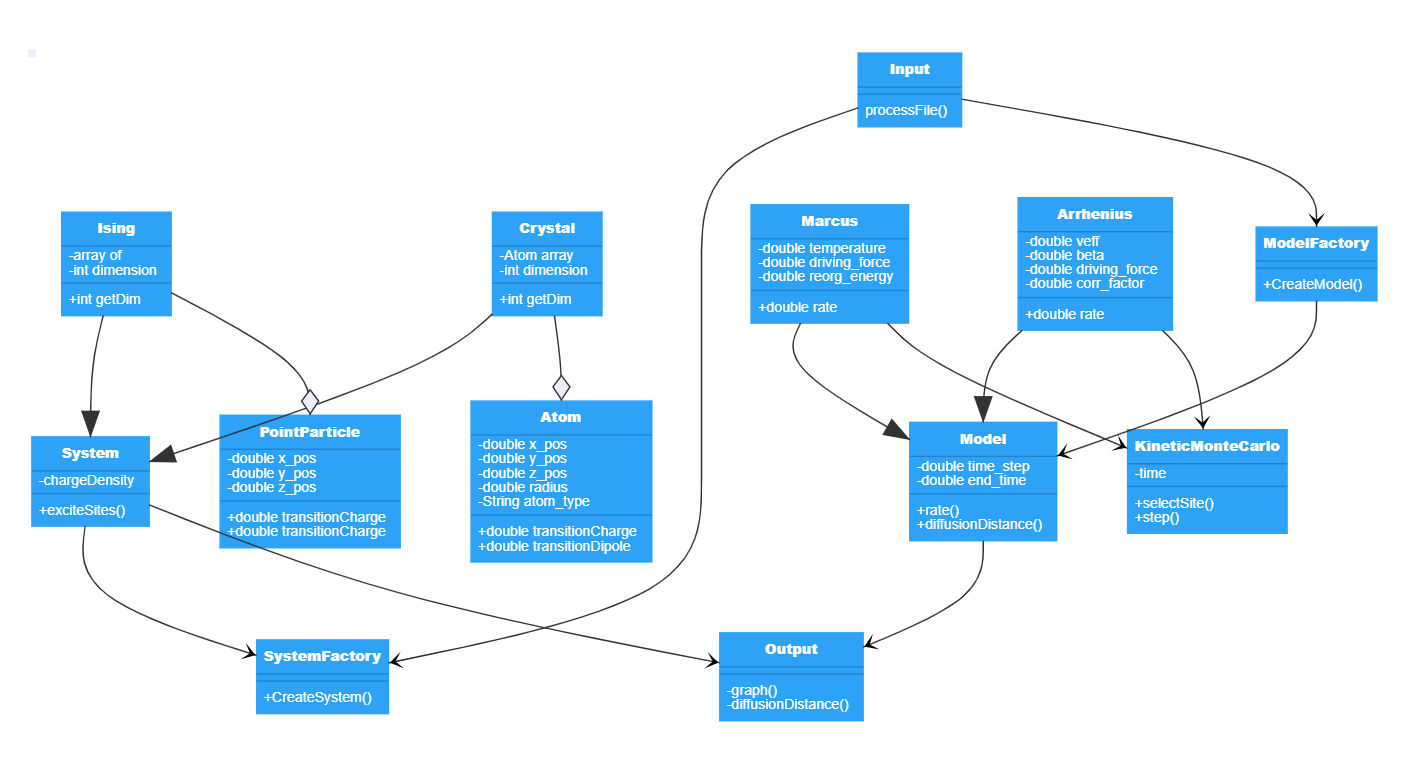
\includegraphics[scale=.25]{uml.png}
    \caption{UML Diagram}
    \label{fig:my_label}
\end{figure}



\subsection{Input}

The inputs for computing the coulombic coupling ($J_{Coul}$), which are the transition dipole moment or the transition charges for a particular excited state, will be obtained using the quantum chemistry package Gaussian 16. The input file with the position vectors of crystalline materials will be imported as .cif file format from Cambridge Crystallographic Data Centre (CCDC). Both of these files are text files, and thus they can be processed using existing packages. From these files and command line inputs, the system and desired model will be determined. As a second option, the user can input a text file with the line "Ising <model name>" or "<model name>", and the program will run a default program.

\subsection{Model}

For evaluating the kinetics of exciton transport in materials, we will examine site hopping models in the adiabatic and nonadiabatic limits. In the non-adiabatic limit, the rate equation is the Marcus rate equation; in the adiabatic limit, the Arrhenius rate equation. These will both be concrete classes of the abstract class Model, which will include a generic rate equation. Additionally, a method for calculating the diffusion distance is included in the abstract class. Both of these models will use the kineticMonteCarlo method to propagate the exciton through space.

\subsection{System}

Any instance of the abstract System class will be an aggregate class of some type of site. The simplest system, the Ising model, is an aggregate of point particles. The other current system is the crystal, which is composed of atoms. These sites all have position, and the aggregate classes keep track of which particles are close to each other. Additionally, the abstract System class will contain a method to excite sites randomly based on either charge density or a random selection process (depending on the presence of single or multiple excitons).

\subsection{Output}

\begin{figure}
    \centering
   \includegraphics[scale=.35]{out2.png}
    \caption{Exciton transport visualization}
    \label{fig:my_label}
\end{figure}

We plan to represent one of our results for our energy migration in materials in the following manner. Figure 2a represents an example of a benzene crystal with the crystalline axis abc. The centroids of each benzene sub-unit will be converted to a simplified ball model (Figure 2b). All the sub-units which are not involved in the energy migration will be removed from the final representation (Figure 2c). The sub-units which take part in the exciton transport will additionally be color coded according to their position vectors from the origin to visualize the depth of the system. 


\section{Estimated Timeline}


31 Oct: Update the preliminary design from the suggestions received from class. Agree on GitHub workflow

3 Nov: Implement a working Monte Carlo simulation for simple atomic model

14 Nov: Updated model to include advanced materials and kinetic models

21 Nov: Integration of visualization capabilities

22-23 Nov: Check in with the AI

30 Nov: Working alpha version

13 Dec: Project completion

\printbibliography

\end{document}  